\section{Algoritmus A*}\label{sec:astar}

Nyní omezíme naše soustředění na případy, kdy hledáme cestu pouze do nějakého konkrétního vrcholu\footnote{"G" od angl. \emph{goal}} $v_G\in V$ (nikoliv do všech, jako tomu bylo doposud). Stále pracujeme s grafy, jejichž hrany mají nezáporné ohodnocení. Všechny dosavadně vysvětlené algoritmy by jistě fungovaly i v tomto případě (při otevírání cílového vrcholu jednoduše vyskočíme z hlavního cyklu). Nabízí se však otázka, zdali nemůžeme znalosti cílového vrcholu nějak využít. Pokud bychom např. hledali nejkratší cestu v mřížce s rozmístěnými překážkami (tj. na některá políčka nelze vstoupit), nejpíše by dávalo smysl upřednostňovat políčka, která jsou blíže cílovému políčku, než ty, která jsou od něj dál.

Mějme bludiště, v němž se nachází hráč (oranžový kruh), jež se může pohybovat libovolným směrem vždy o jedno pole, přičemž cílovým pole se nachází vpravo dole (červeně vyznačené). Situaci lze vidět na obrázku \ref{fig:mrizka}. Takovou situaci můžeme znázornit pomocí grafu, kde každá hrana má váhu 1, popř. lze použít neohodnocený graf.
\begin{figure}[h]
    \centering
    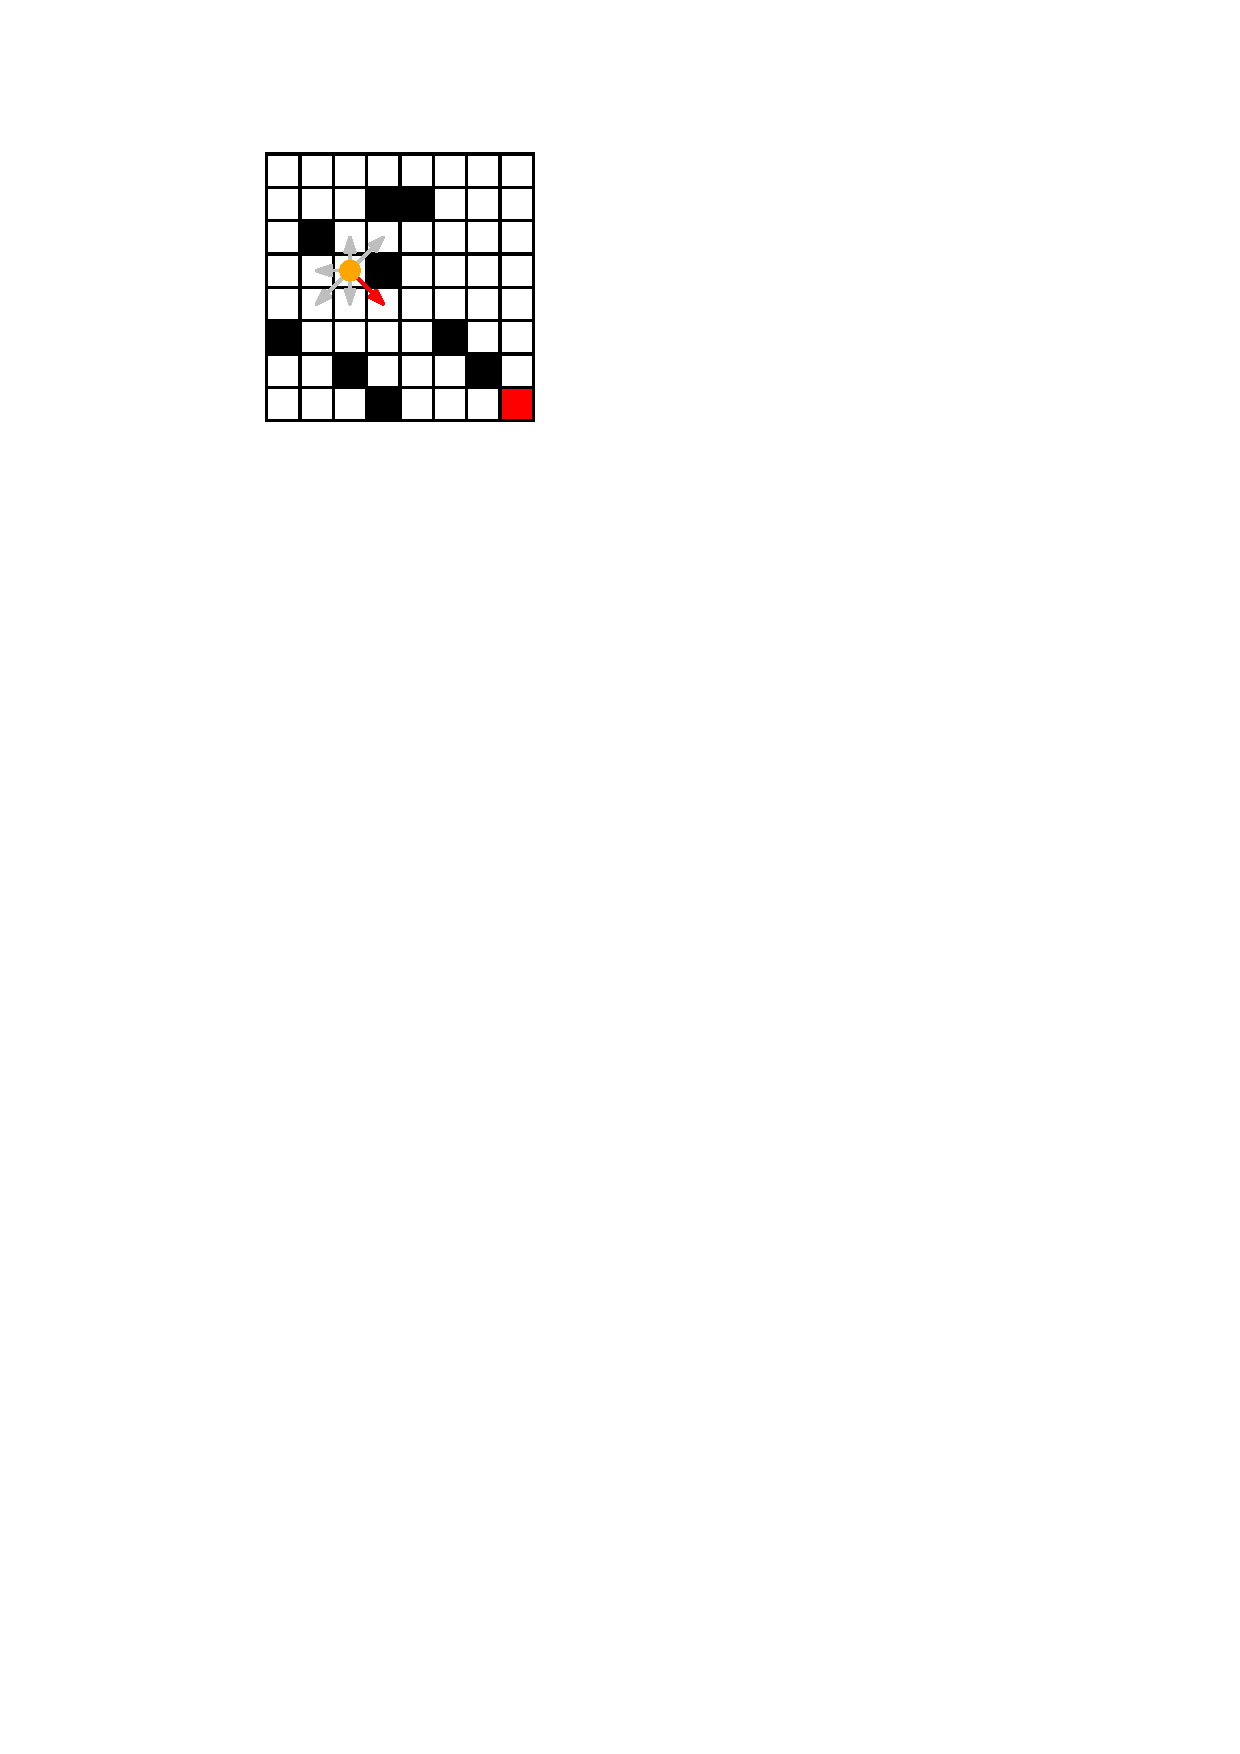
\includegraphics[scale=1.2]{01-grafalgo/images/ch01_mrizka.pdf}
    \caption{Mřížka a optimální směr pohybu hráče.}
    \label{fig:mrizka}
\end{figure}
Pokud bychom aplikovali např. BFS, či Dijkstrův algoritmus, prozkoumali bychom postupně všechny směry (šipky) stejně. Je však zřejmé, že nejvýhodnější je vydat směrem vyznačeným červeně, neboť je nejblíže cíli. V roce 1968 tak přišli Peter Hart, Nils Nilsson a Bertam Raphael s úpravou původního Dijkstrova algoritmu, která nese název A*.

Myšlenka je stále stejná, avšak nyní budeme vybírat vrcholy podle hodnoty $D(v)+\psi(v)$ (místo pouhého $D(v)$), kde $\psi$ je tzv. \emph{heuristická funkce} nebo zkráceně \emph{heuristika}, která slouží jako \emph{odhad vzdálenosti od cílového vrcholu} v grafu (viz obrázek \ref{fig:astar_heuristika}).
\begin{figure}[h]
    \centering
    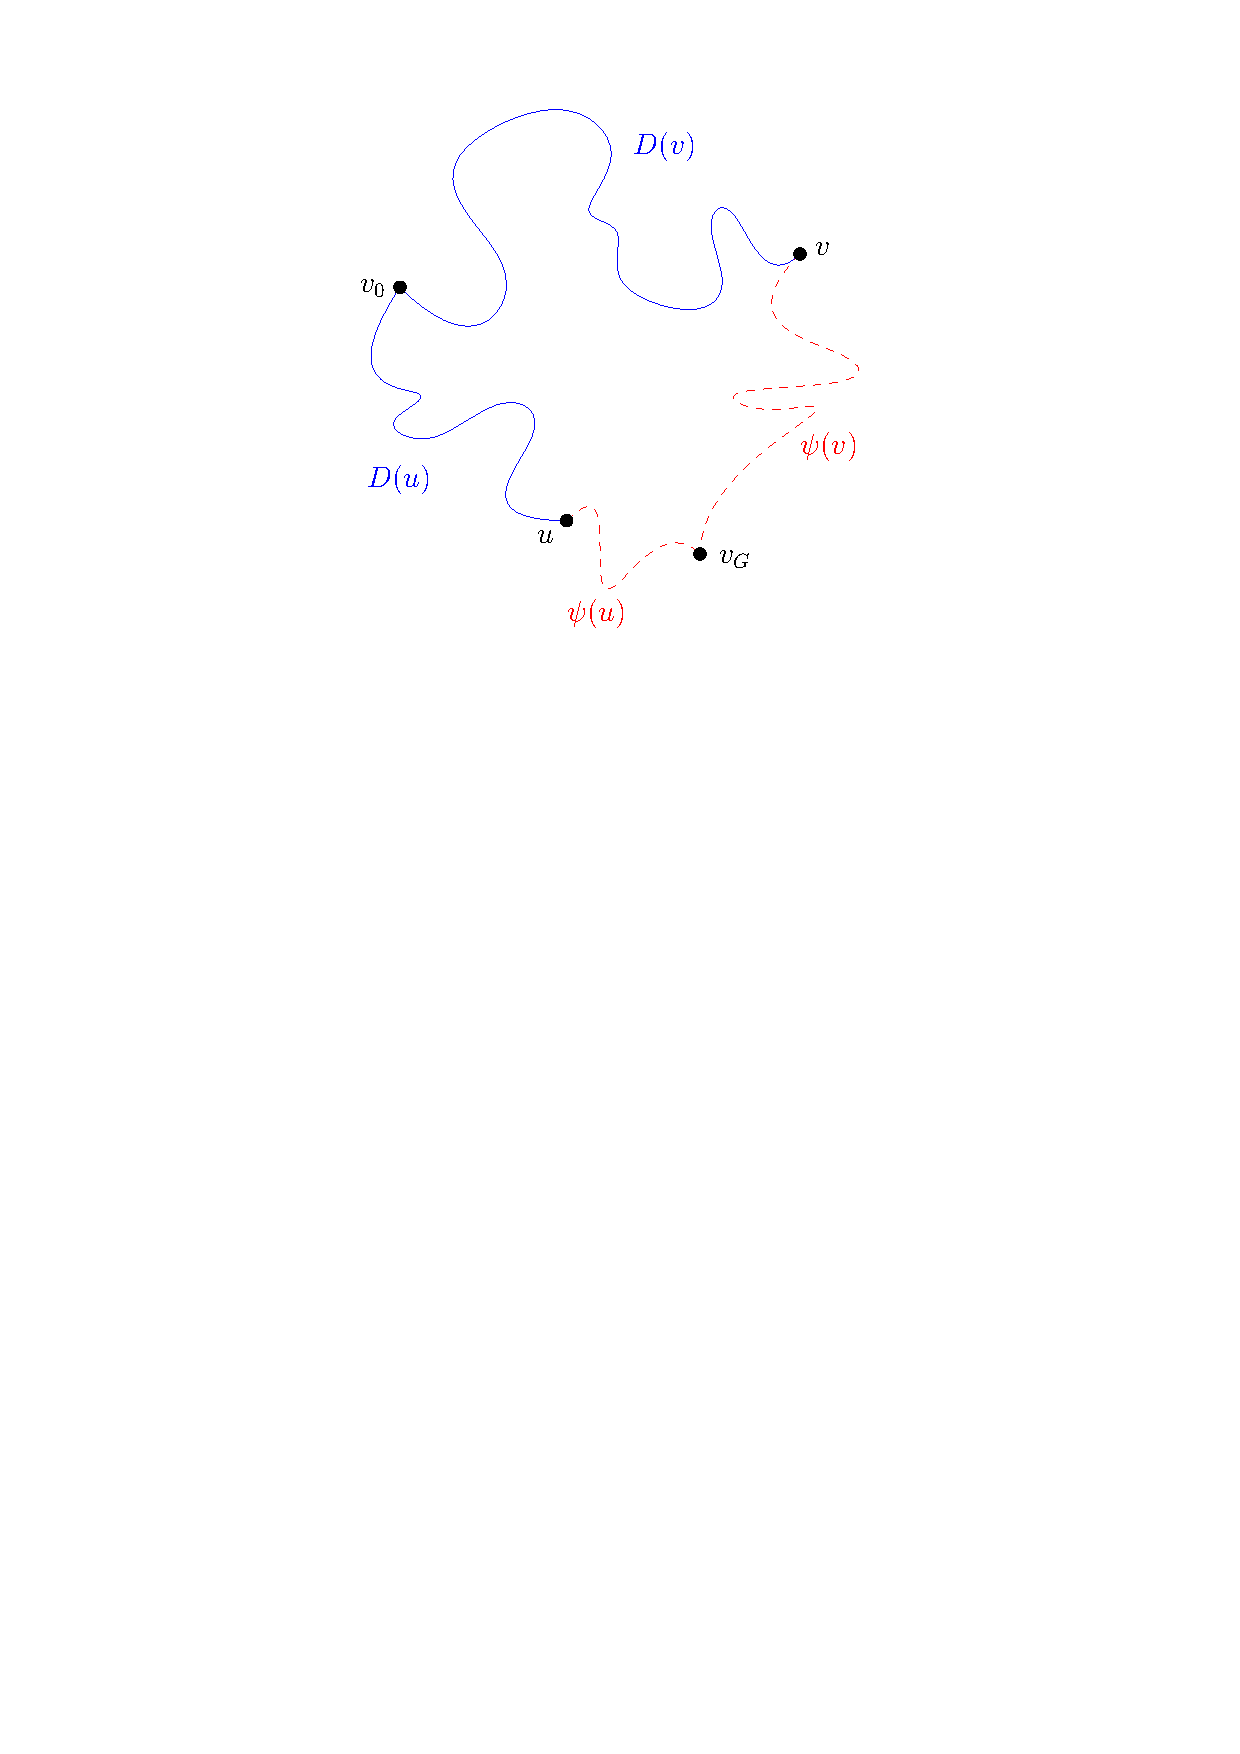
\includegraphics[scale=\graphimgsize]{01-grafalgo/images/ch01_astar_heuristika.pdf}
    \caption{Znázornění heuristické funkce $\psi$.}
    \label{fig:astar_heuristika}
\end{figure}
Součtu $D(v)+\psi(v)$ budeme říkat tzv. \emph{f-skóre}\footnote{V jiných textech, převážně anglických, se někdy používá pro heuristiku označení $h$ a pro vzdálenost označení $g$, tzv. \emph{g-skóre}, tj. $f(v)=g(v)+h(v)$.}, značíme $f(v)$. V každé iteraci tak budeme vybírat vrchol s nejnižším $f$-skóre, k čemuž lze opět použít pole, nebo binární haldu.

Oproti Dijkstrově algoritmu tedy skutečně nenastává moc změn, akorát je potřeba si zvlášť uchovávat hodnoty $f$-skóre.
\begin{pseudo}{A*}[Nezáporně ohodnocený graf $G=(V,E)$ a počáteční vrchol $v_0\in V$.][Vzdálenost $v_0$ od $v_G$.]
    \Comment{Inicializace}
    \begin{For}{všechny vrcholy $v\in V$}
        $stav(v)\gets$ \textit{nenalezený}\\
        $D(v)\gets\infty,\,f(v)\gets\infty$\\
    \end{For}
    $stav(v_0)\gets$ \textit{otevřený}\\
    $D(v_0)\gets 0,\,f(v_0)\gets\psi(v_0)$\\
    \begin{While}{existují otevřené vrcholy}
        $v\gets$ otevřený vrchol s nejmenším $f$-skóre\\\\
        \begin{If}{$v=v_G$}
            \Return{$D(v_G)$}\\
        \end{If}
        \begin{For}{všechny sousedy $w\in V$ vrcholu $v$}
            \Comment{Našli jsme lepší cestu}
            \begin{If}{$D(v)+\ell(v,w)<D(w)$}
                $D(w)\gets D(v)+\ell(v,w)$\\
                $f(w)\gets D(v)+\ell(v,w)+\psi(w)$\\
                $stav(w)\gets$ \textit{otevřený}
            \end{If}
        \end{For}
        $stav(v)\gets$ \textit{uzavřený}
    \end{While}
    \Return{$D(v_G)$}
\end{pseudo}

\subsubsection{Správnost algoritmu A*}

Podobně jako u Dijkstrova algoritmu i zde platí, že při výběru (tj. otevírání) vrcholu $v$ odpovídá $D(v)$ délce nejkratší cesty. Argument pro tuto skutečnost je podobný. Předpokládejme, že otevíráme nějaký vrchol $v$, přičemž hodnota $D(v)$ je větší, než je skutečná délka nejkratší cesty. Pak existuje nějaký sousední vrchol $u$ vrcholu $v$, přes nějž nutně vede nejkratší cesta do $v$, tj. platí $D(u)+\ell(u,v)<D(v)$ (viz obrázek \ref{fig:astar_kratsi_cesta}).
\begin{figure}[h]
    \centering
    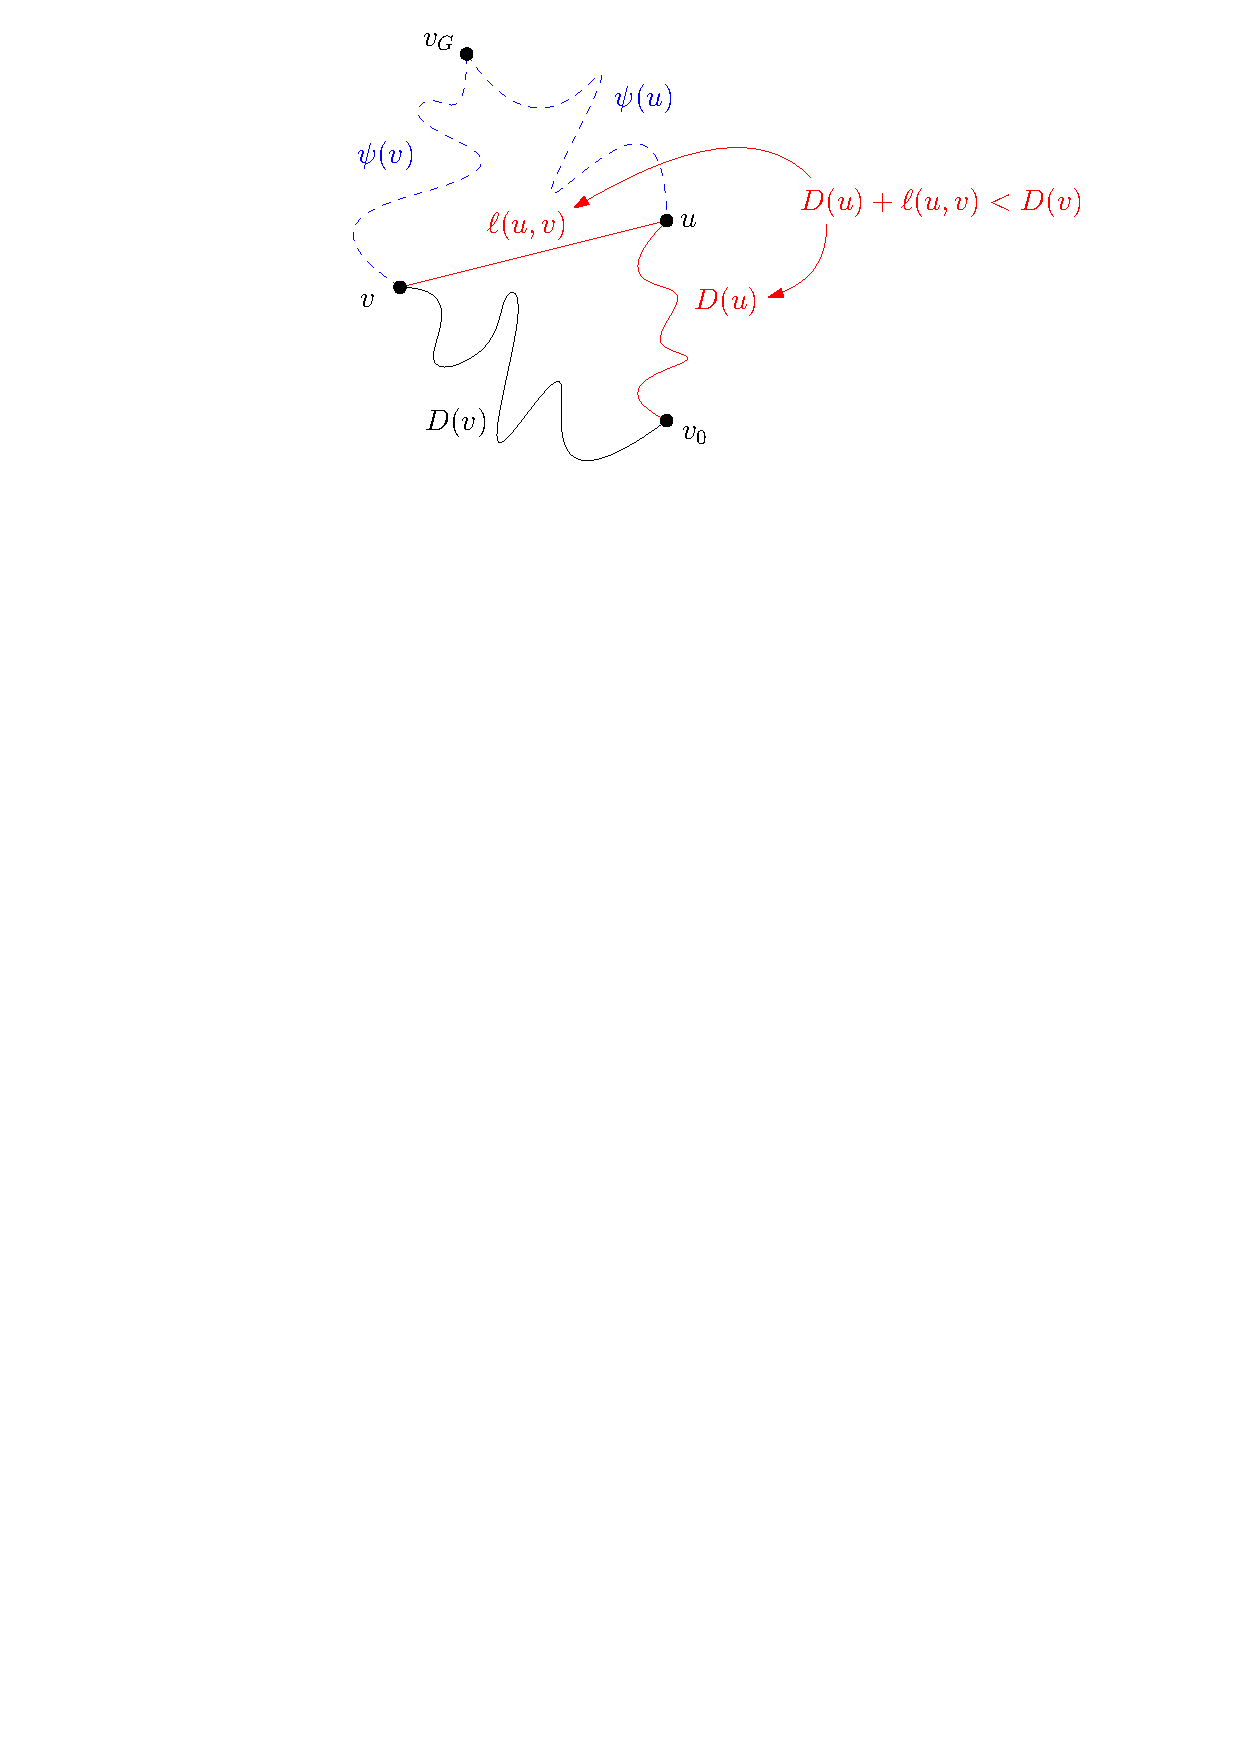
\includegraphics[scale=\graphimgsize]{01-grafalgo/images/ch01_astar_kratsi_cesta.pdf}
    \caption{Situace při výběru vrcholu $v$ při heuristice $\psi$, kdy $D(v)$ neodpovídá délce nejkratší cesty.}
    \label{fig:astar_kratsi_cesta}
\end{figure}
Jak to bude s $f$-skóre vrcholu $v$? Těžko říci. Co vůbec víme o funkci $\psi$? Zatím jsme si nespecifikovali žádné vlastnosti, které bychom od ní očekávali. Ukazuje se však, že $\psi$ si libovolně zvolit nemůžeme. Naše heuristika musí být v jistém smyslu "rozumná". Pokud se vydáme z vrcholu $u$ po hraně do vrcholu $v$ a z něj poté do cílového vrcholu $v_G$, určitě výsledná cesta bude alespoň tak dlouhá, jako nejkratší cesta z $u$ do $v_G$. To samé by mělo platit i pro náš odhad vzdáleností\footnote{Tomu se obecně říká tzv. \emph{trojúhelníková nerovnost}. Pro libovolnou trojici vrcholů platí $d(u,v)\leqslant d(u,w)+d(w,v)$, kde $d$ značí vzdálenost daných vrcholů v grafu $G$.}, tedy $\psi(u)\leqslant\ell(u,v)+\psi(v)$.

Pokud tedy budeme předpokládat, že $\psi$ splňuje výše zmíněnou vlastnost, musí pak platit následující:
\[f(u)=D(u)+\overbrace{\psi(u)}^{\leqslant\ell(u,v)+\psi(v)}\leqslant \underbrace{D(u)+\ell(u,v)}_{<D(v)}+\psi(v)<D(v)+\psi(v)=f(v).\]
Z toho je ale již vidět, že $f(u)<f(v)$, tedy $u$ musí mít nižší $f$-skóre než $v$. Tzn. algoritmus A* by upřednostnil vrchol $u$ před $v$.

Upozorněme zde na fakt, že náš předpoklad o heuristice je velmi důležitý, neboť pokud bychom si zvolili heuristiku nevhodně, algoritmus již fungovat nebude a obecně může dojít k tomu, že nějaký z vrcholů vybereme "předčasně".

\begin{remark}
    \begin{itemize}
        \item Všimněme si, že Dijkstrův algoritmus je speciálním případem algoritmu A*. Stačí pro všechny vrcholy $v$ položit\footnote{Lze zvolit klidně i obecnou konstantu $c\in\R$, tj. $\psi(v)=c$.} $\psi(v)=0$.
        \item Je dobré dodat, že heuristiku bychom měli být schopni pro každý vrchol spočítat co nejrychleji, nejlépe v konstantním čase, tj. $\bigO{1}$.
    \end{itemize}
\end{remark}

Rozbor časové složitosti zde vynecháme. Je totiž silně závislá na tom, jakou heuristiku $\psi$ si zvolíme. Při vhodné volbě doběhne A* zpravidla rychleji oproti Dijkstrově algoritmu. Může se však také stát, že $\psi$ zvolíme nevhodně (i přesto, že splňuje trojúhelníkovou nerovnost výše), a algoritmus nakonec poběží déle.

\subsubsection{Ukázky heuristických funkcí}

Zbývá zodpovědět otázku, jakou heuristiku tedy použít? Odpověď není zcela jednoznačná, neboť záleží na situaci. Vraťme se opět k příkladu s bludištěm, kdy začínáme na určitém políčku a snažíme se dostat do cílového, přičemž hráč se smí pohybovat všemy směry vždy o jedno pole. Políčka identifikujeme podle jejich souřadnic, tj. dvojice $(x,y)$.

Jednou možností je tzv. \emph{eukleidovská vzdálenost}. Ta je pro libovolnou dvojici bodů v rovině $X=(x_1,y_1)$ a $Y=(x_2,y_2)$ definována jako
\[\sqrt{(x_1-x_2)^2+(y_1-y_2)^2}.\]
V případě cílového políčka známe jeho souřadnice, takže můžeme snadno vypočítat eukleidovskou vzdálenost libovolného políčka od cílového. To lze použít jako heuristiku\footnote{Dokonce bychom mohli použít jako heuristiku pouze výraz pod odmocninou, tj. $(x_1-x_2)^2+(y_1-y_2)^2$.}, označme si ji $\psi_E$. Situaci lze sledovat na obrázku \ref{fig:astar_bludiste_euclid}, kde šedě je vyznačena nejkratší cesta do pole se souřadnicemi $(x,y)$.
\begin{figure}[h]
    \centering
    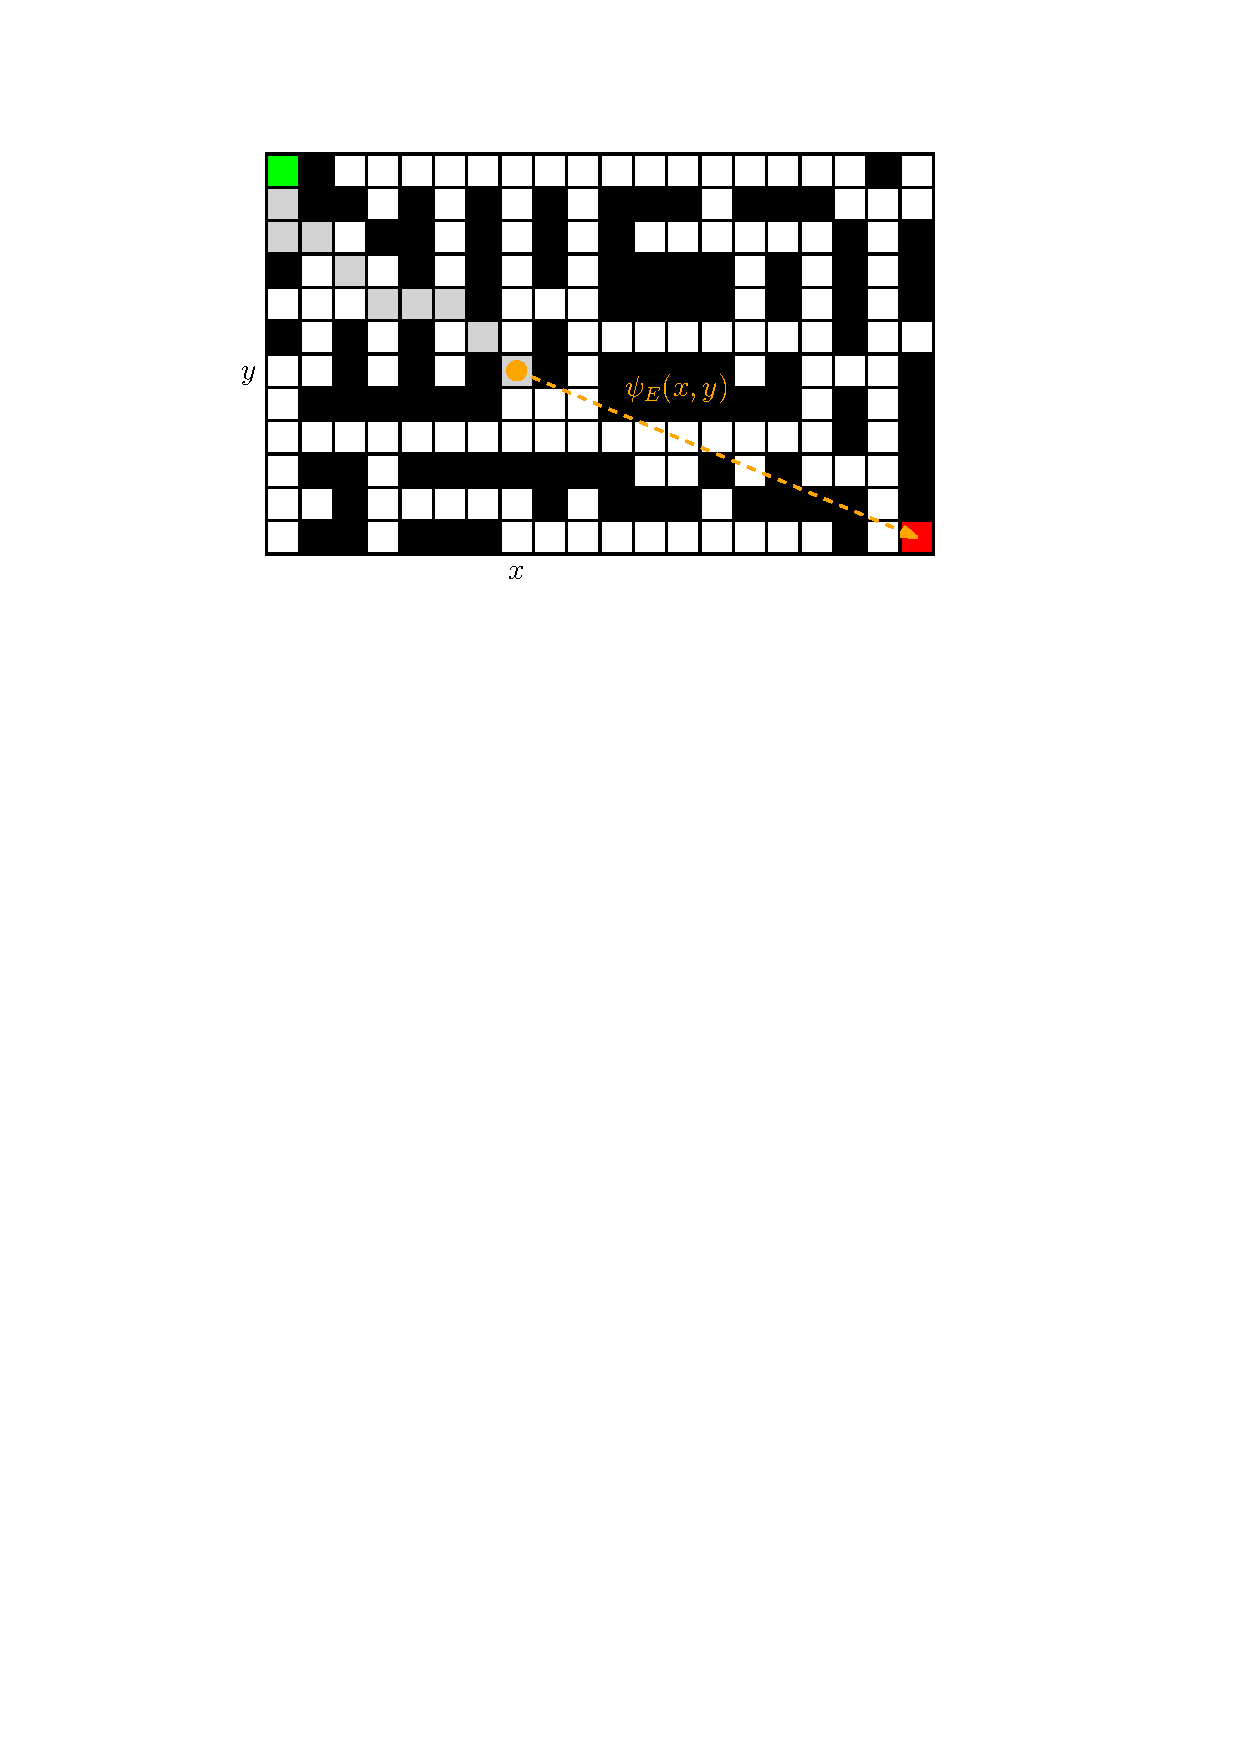
\includegraphics[scale=\graphimgsize]{01-grafalgo/images/ch01_astar_mrizka_euclid.pdf}
    \caption{Příklad bludiště s eukleidovskou heuristikou.}
    \label{fig:astar_bludiste_euclid}
\end{figure}
Pokud bychom však pracovali s bludištěm, kde se \emph{nelze pohybovat po diagonálách} nebo by nám to pravidla neumožňovala, můžeme výpočet heuristické funkce nahradit něčím jednodušším. V tomto ohledu se pak často využívá tzv. \emph{manhattanská vzdálenost} (označme $\psi_M$) definovaná vztahem
\[\abs{x_1-x_2}+\abs{y_1-y_2}.\]
\begin{figure}[h]
    \centering
    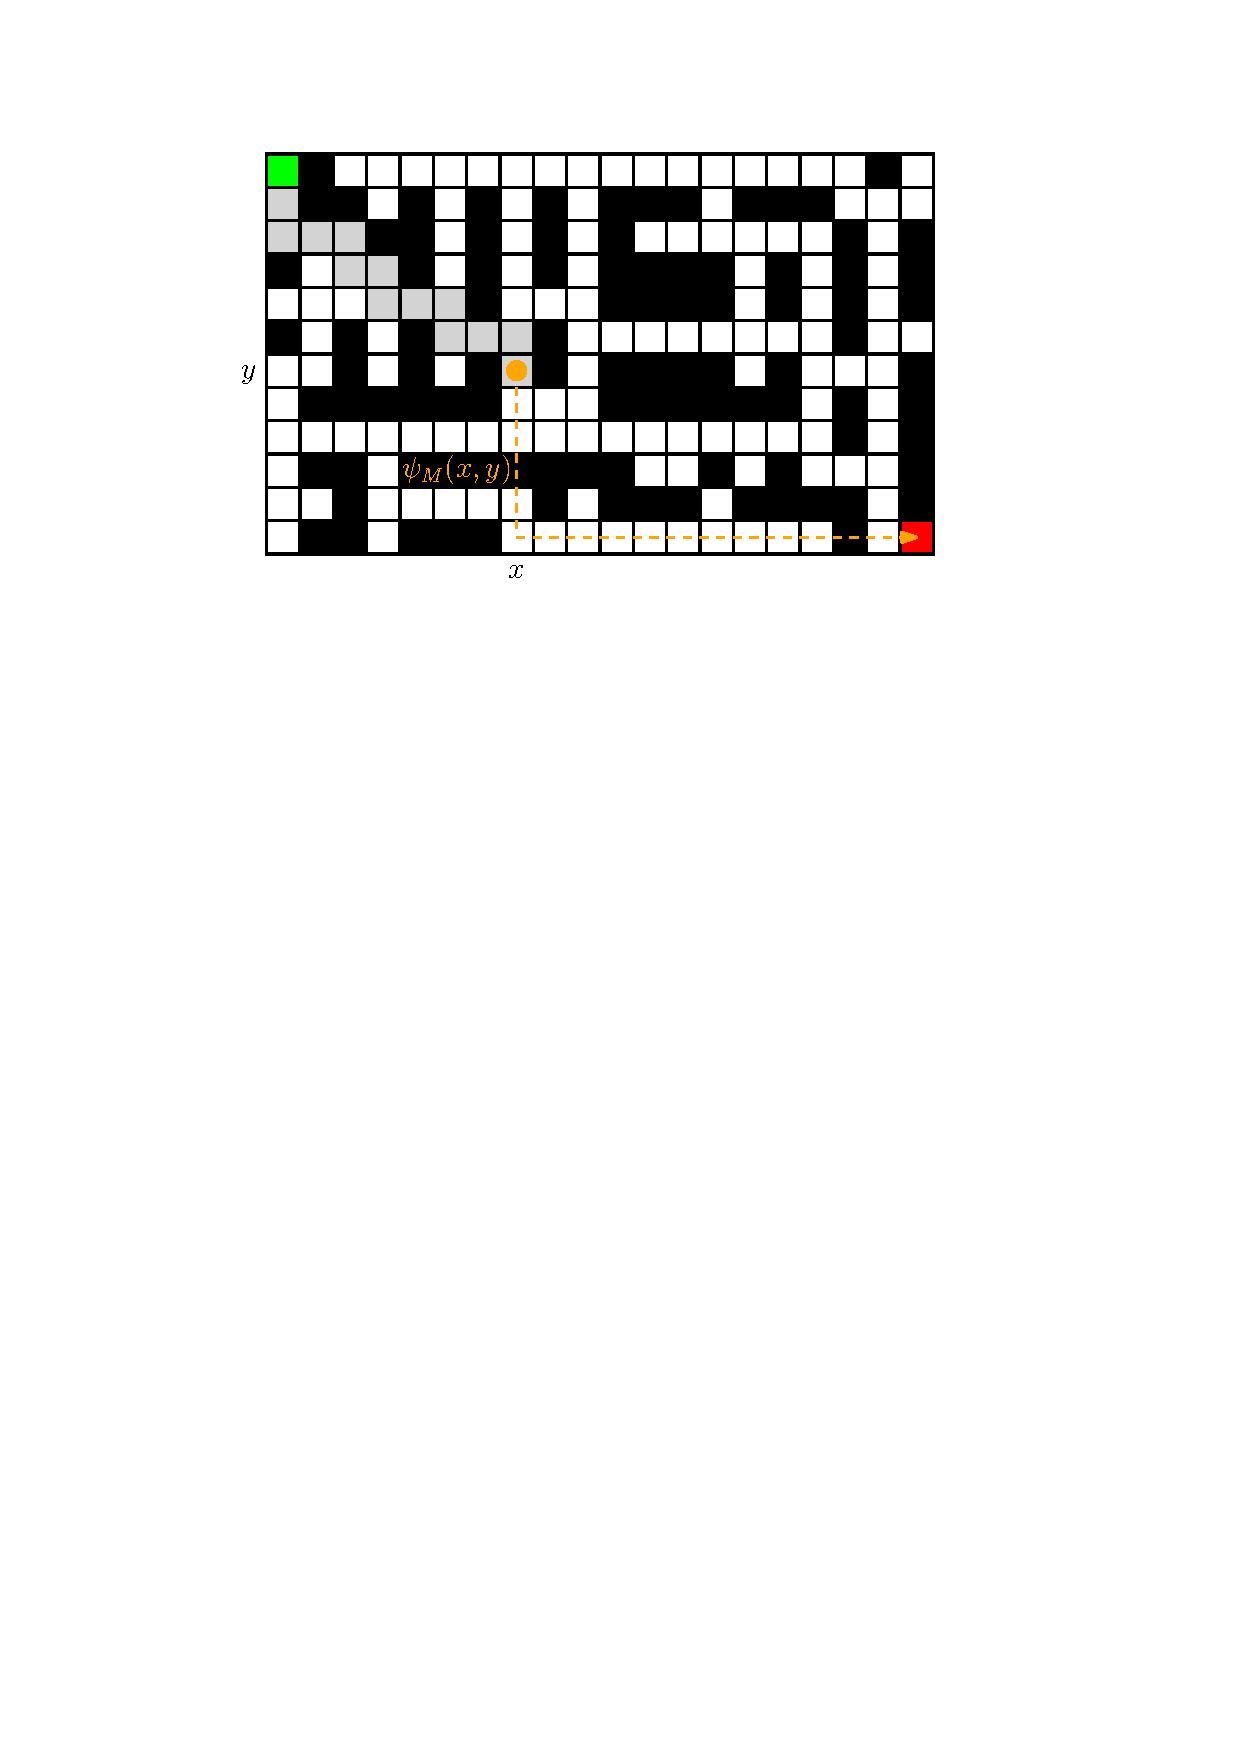
\includegraphics[scale=\graphimgsize]{01-grafalgo/images/ch01_astar_mrizka_manhattan.pdf}
    \caption{Příklad bludiště s manhattnskou heuristikou.}
    \label{fig:astar_bludiste_manhattan}
\end{figure}
Stejně jako eukleidovská vzdálenost, i manhattanská vzdálenost splňuje trojúhelníkovou nerovnost. Její výhodou je nižší náročnost při výpočtu (výpočet odmocniny\footnote{V mnoha případech, např. v některých starších videohrách jako Quake III, se vývojáři snažili vyhýbat výpočtu odmocniny, nebo volili některé sofistikovanější výpočty, které byly rychlé a poskytovaly uspokojivý odhad hledané hodnoty.} je již trochu pomalejší) a to hlavně z důvodu, že pracujeme vždy s celými čísly. Její nevýhodou však může být, že oproti eukleidovské vzdálenosti nabývá větších hodnot.